\chapter{Evaluation}\label{chap:evaluation}

Clearly not every project has empirical components (in particular in mathematics or theoretical topics) -- though many do. So in case you were coding anything and conducted an empirical evaluation, this is where you should report the results.

The following sections are, as for the rest of this template, just \emph{suggestions}. They might fit to your work, or they don't. Discuss this with your supervisor(s).

% Due to the small size of the subsections here, I didn't use includes in the code.
% In your case, however, those subsections are likely larger and might thus justify
% using imports. As before: One file per subsection.

\section{Benchmark Set}

This is where you describe the set of benchmarks that you use for testing your hypothesis empirically. Some ideas on what information you could convey:

\begin{itemize}
  \item What's the origin of your benchmarks, where are they from?
  \item What benchmark set did you use \emph{exactly}, i.e., can you explain what they are/mean?
  \item Why did you choose these benchmarks, and not others? I.e., why are they appropriate for your evaluation? Are they maybe some sort of ``standard'' and thus also used by others?
  \item Could you have chosen other benchmarks? If so, which? Why didn't you do so? (Could this maybe form future work?)
\end{itemize}

In nutshell, just tell everything interesting about the set of benchmarks selected.


\section{Evaluated Software}

This is where you would describe all software or algorithms etc. that you test. For example, if later you have tables or plots with some abbreviations to denote algorithms or specific configurations of your algorithm(s), then this would be the place to define and explain them. So, all these abbreviations/acronyms or software names should be explained/introduced here, and explained in sufficient detail.

Furthermore, in most works you might not only test your own software/contributions, but you might compare it against software from the literature. If possible, then this is certainly good style, as you are usually not the first to tackle a certain problem: Others have attempted this before. So you should compare your performance against performance of the current/previous state of the art. Therefore, this software should be listed here as well. You might potentially have explained these other ``competitors'' before in the related work section, but there you focused on their scientific approach. Here you would list their software names and configurations, and otherwise reference back to the related work section. Explain why you compare against this software, and maybe mention other related software as well, explaining why you did not compare against it.


\section{Hardware Setup}

This section is supposed to explain all details on how to run the above-mentioned software, so that others could reproduce it, or at least can interpret your results appropriately. This is usually rather short.

On what computer was the experiment run? I.e., 
\begin{itemize}
  \item What was the Operating System? (Name and version number.)
  \item What processor (CPU) was used, and how many? Single-core, or Multi-core? (In some disciplines, such as AI planning, only a single CPU is used, even if the processor has multiple cores.) Was GPU power used as well? If so, which?
  \item How much RAM was made available? (Note that this is typically different from the RAM the hardware has available, as we can reserve a specific amount to processes, which is lower than the total amount physically available.)
  \item How much runtime did you grant your processes? How did you measure it? Did you take ``walltime'' or ``CPU time''? If you don't know what this means, google it! Explaining it might also be appropriate.
  \item Was your system a VM, running within another operating system (e.g., Linux within Windows), in a cluster, on a server, a personal laptop, etc.?
\end{itemize}

In a nutshell, you should simply report anything that will enable your reader to interpret your numbers that you are going to report later. 


\section{Empirical Results}

This is the ``core'' of your section: Here you report all your findings. 

A \emph{very important} observations is that you will have to report on \emph{two} things, where some might forget the second, although this is actually the more important item:

\begin{itemize}
  \item Plain data. This is the raw data you obtained, reported in tables or plots or the like. E.g. which problems did you solve in the available time? How well did you classify the input correctly? (This is clearly content-specific.) Make sure to report your data in an appropriate way, enabling the reader to easily grasp what the data is supposed to show. It is important to discuss this early on with your supervisor, as he/she likely knows better how to appropriately report on your findings. (Also don't forget to look into important literature working on similar topics.)
  \item Interpretation. This is what you can infer from your results. Did the approach work well, or did it not? If it worked well, then to which extent? Does it \emph{always} perform best (unlikely!), or is there a subset of benchmarks on which it worked well? If so, why? What's special about this subject making the approach work well there? Do your findings raise further questions and thus directions for future research/investigations? Please do not worry if your results are objectively bad. Certainly bad results can not be published, but you can still obtain very high marks. It is your job to evaluate how well (or how badly!) your approach worked, and it's (likely) not your fault if it did not. So making up ridiculous reasons why the results are great although they are clearly not is anti-scientific and will thus make an incredibly bad impression and penalized mark-wise. Simply objectively and truthfully report the findings -- this is science. If the results are bad, can you explain or at least hypothesize why? (This would prove your high level of understanding.) Can you form future work based on your findings?
\end{itemize}

When reporting your results using graphs and plots, make sure to provide all information necessary to interpret the data, e.g., axis and graph labeling (cf.~Figure~\ref{fig:xkcd}).

  \begin{figure}[bh!]
  \floatbox[{\capbeside\thisfloatsetup{capbesideposition={left,top},capbesidewidth=.5\textwidth}}]{figure}[\FBwidth]
  {\caption{A graph illustrating the importance of axis and graph labeling. (Graphic taken from \url{https://xkcd.com/252/}.)\label{fig:xkcd}}}
  {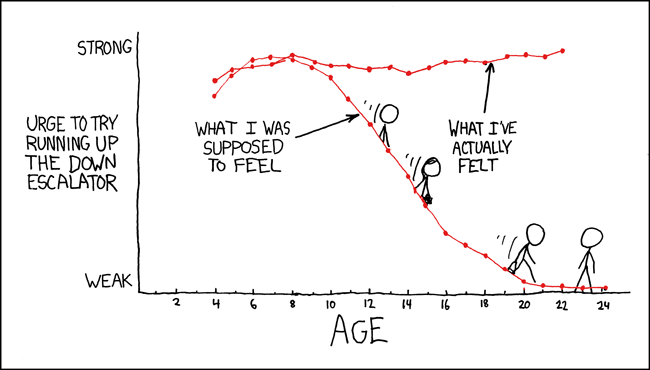
\includegraphics[width=.45\textwidth]{figures/escalators.png}}
  \end{figure}

When you print tables, it's good style to highlight the best results in bold. Also use the \textsc{booktabs} package for nicely formatted tables, as explained in the previous section on \LaTeX{} advice. (That's not a must, but it will simply look much nicer!)